%iffalse
\let\negmedspace\undefined
\let\negthickspace\undefined
\documentclass[journal,12pt,onecolumn]{IEEEtran}
\usepackage{cite}
\usepackage{amsmath,amssymb,amsfonts,amsthm}
\usepackage{algorithmic}
\usepackage{graphicx}
\usepackage{textcomp}
\usepackage{xcolor}
\usepackage{txfonts}
\usepackage{listings}
\usepackage{enumitem}
\usepackage{enumitem,multicol}
\usepackage{mathtools}
\usepackage{gensymb}
\usepackage{comment}
\usepackage[breaklinks=true]{hyperref}
\usepackage{tkz-euclide} 
\usepackage{listings}
\usepackage{gvv}                                        
%\def\inputGnumericTable{}                                 
\usepackage[latin1]{inputenc}                                
\usepackage{color}                                            
\usepackage{array}                                            
\usepackage{longtable}                                       
\usepackage{calc}                                             
\usepackage{multirow}                                         
\usepackage{hhline}                                           
\usepackage{ifthen}                                           
\usepackage{lscape}
\usepackage{tabularx}
\usepackage{array}
\usepackage{float}
\usepackage[american,siunitx]{circuitikz}
\usetikzlibrary{arrows,shapes,calc,positioning}
\usepackage{pgfplots}


\newtheorem{theorem}{Theorem}[section]
\newtheorem{problem}{Problem}
\newtheorem{proposition}{Proposition}[section]
\newtheorem{lemma}{Lemma}[section]
\newtheorem{corollary}[theorem]{Corollary}
\newtheorem{example}{Example}[section]
\newtheorem{definition}[problem]{Definition}
\newcommand{\BEQA}{\begin{eqnarray}}
\newcommand{\EEQA}{\end{eqnarray}}
\newcommand{\define}{\stackrel{\triangle}{=}}
\theoremstyle{remark}
\newtheorem{rem}{Remark}
\pgfplotsset{compat=1.18}

% Marks the beginning of the document
\begin{document}
\bibliographystyle{IEEEtran}
\vspace{3cm}

\title{PH-2019}
\author{EE24Btech11022 - Eshan Sharma}
\maketitle

\renewcommand{\thefigure}{\theenumi}
\renewcommand{\thetable}{\theenumi}



\begin{enumerate}
\item Consider the motion of a particle along the x-axis in a potential $V(x) = F|x|$. Its ground state energy $E_0$ is estimated using the uncertainty principle. Then $E_0$ is proportional to
\begin{multicols}{4}
	\begin{enumerate}
		\item $F^{\frac{1}{3}}$
		\item $F^{\frac{1}{2}}$
		\item $F^{\frac{2}{5}}$
		\item $F^{\frac{2}{3}}$
	\end{enumerate}
\end{multicols}

\item A 3-bit analog-to-digital converter is designed to digitize analog signals ranging from 0 V to 10 V. For this converter, the binary output corresponding to an input of 6 V is
\begin{multicols}{4}
	\begin{enumerate}
		\item 011
		\item 101
		\item 100
		\item 010
	\end{enumerate}
\end{multicols}

\item The Hamiltonian operator for a two-level quantum system is $H = \begin{pmatrix} E_1 & 0 \\ 0 & E_2 \end{pmatrix}$. If the state of the system at $t = 0$ is given by $\lvert \psi (0) \rangle = \frac{1}{\sqrt{2}} \begin{pmatrix} 1 \\ 1 \end{pmatrix}$, then $\lvert \langle \psi (0) | \psi (t) \rangle \rvert ^2$ at a later time $t$ is
\begin{multicols}{2}
	\begin{enumerate}
		\item $\frac{1}{2} \left( 1 + e^{-(E_1 - E_2)t/\hbar} \right)$
		\item $\frac{1}{2} \left( 1 - e^{-(E_1 - E_2)t/\hbar} \right)$
		\item $\frac{1}{2} \left( 1 + \cos[(E_1 - E_2)t/\hbar] \right)$
		\item $\frac{1}{2} \left( 1 - \cos[(E_1 - E_2)t/\hbar] \right)$
	\end{enumerate}
\end{multicols}

\item A particle of mass $m$ moves in a lattice along the x-axis in a periodic potential $V(x) = V(x + d)$ with periodicity $d$. The corresponding Brillouin zone extends from $-k_0$ to $k_0$, with these two $k$-points being equivalent. If a weak force $F$ in the x-direction is applied to the particle, it starts a periodic motion with time period $T$. Using the equation of motion $F = \frac{dp_{\text{crystal}}}{dt}$ for a particle moving in a band, where $p_{\text{crystal}}$ is the crystal momentum of the particle, the period $T$ is found to be (h is Planck constant)
\begin{multicols}{4}
	\begin{enumerate}
		\item $\sqrt{\frac{2md}{F}}$
		\item $2 \sqrt{\frac{2md}{F}}$
		\item $\frac{2h}{Fd}$
		\item $\frac{h}{Fd}$
	\end{enumerate}
\end{multicols}
\item Consider a potential barrier \( V(x) \) of the form:

\begin{center}
	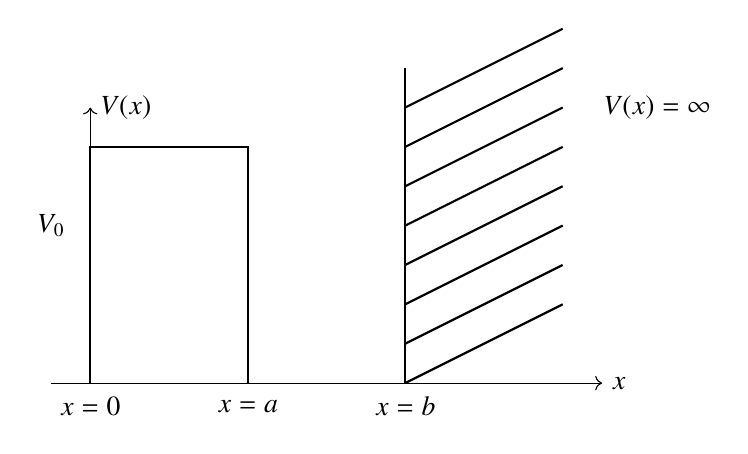
\begin{tikzpicture}
	% Potential barrier V(x)
	\draw[thick] (0,0) -- (0,3) -- (2,3) -- (2,0); % Barrier from x=0 to x=a
	\draw[thick] (4,0) -- (4,4); % Line at x=b representing V(x) = infinity
	
	% Darker angled lines from x-axis and from x=b
	\foreach \y in {0, 0.5, 1, 1.5, 2, 2.5, 3, 3.5} {
		\draw[thick] (4,\y) -- ++(2,1); % Adding lines from x-axis up to x=b
	}
	
	% Axis and labels
	\draw[->] (-0.5,0) -- (6.5,0) node[right] {$x$};
	\node at (0,-0.3) {$x=0$};
	\node at (2,-0.3) {$x=a$};
	\node at (4,-0.3) {$x=b$};
	\draw[->] (0,0)--(0,3.5) node[right] {$V(x)$};
	\node at (-0.5,2) {$V_0$};
	\node at (7.2,3.5) {$V(x) = \infty$};
\end{tikzpicture}

\end{center}


where \( V_0 \) is a constant. For particles of energy \( E < V_0 \) incident on this barrier from the left, which of the following schematic diagrams best represents the probability density \( |\psi(x)|^2 \) as a function of \( x \).

\begin{multicols}{2}
	\begin{enumerate}
		\item
		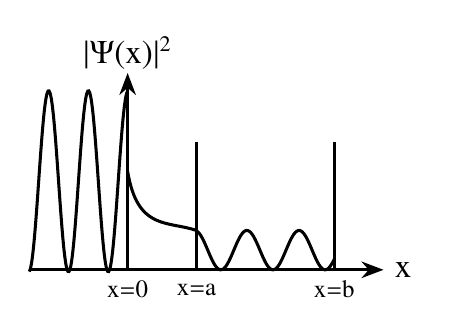
\begin{tikzpicture}[scale=0.5]
			\tikzstyle{every node}=[font=\large]
			\draw [line width=1.1pt, ->, >=Stealth] (11.75,12.75) -- (20.75,12.75);
			\draw [line width=1.1pt, ->, >=Stealth] (14.25,12.75) -- (14.25,17.75);
			\draw [line width=1.1pt, short] (16,12.75) -- (16,16);
			\draw [line width=1.1pt, short] (19.5,12.75) -- (19.5,16);
			\node [font=\small] at (19.5,12.25) {x=b};
			\node [font=\small] at (14.25,12.25) {x=0};
			\node [font=\small] at (16,12.25) {x=a};
			\node [font=\large] at (21.25,12.75) {x};
			\node [font=\large] at (14.25,18.25) {$\mid$$\Psi$(x)$\mid^{2}$};
			\draw[domain=11.75:14.25,samples=100,smooth, line width=1.1pt] plot (\x,{2.3*sin(6.22*\x r -11.75 r ) +15});
			\draw[domain=16:19.5,samples=100,smooth, line width=1.1pt] plot (\x,{0.5*sin(4.74*\x r -17.5 r ) +13.25});
			\draw [line width=1.1pt, short] (14.25,15.25) .. controls (14.5,13.75) and (15.25,14) .. (16,13.75);
		\end{tikzpicture}
		
		\item
		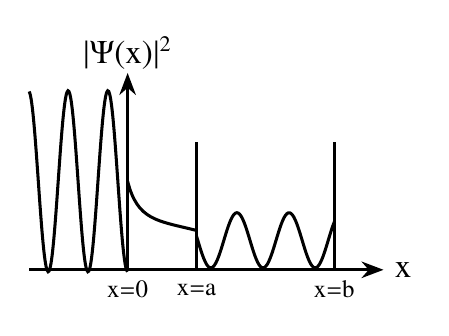
\begin{tikzpicture}[scale=0.5]
			\tikzstyle{every node}=[font=\large]
			\draw [line width=1.1pt, ->, >=Stealth] (11.75,12.75) -- (20.75,12.75);
			\draw [line width=1.1pt, ->, >=Stealth] (14.25,12.75) -- (14.25,17.75);
			\draw [line width=1.1pt, short] (16,12.75) -- (16,16);
			\draw [line width=1.1pt, short] (19.5,12.75) -- (19.5,16);
			\node [font=\small] at (19.5,12.25) {x=b};
			\node [font=\small] at (14.25,12.25) {x=0};
			\node [font=\small] at (16,12.25) {x=a};
			\node [font=\large] at (21.25,12.75) {x};
			\node [font=\large] at (14.25,18.25) {$\mid$$\Psi$(x)$\mid^{2}$};
			\draw[domain=11.75:14.25,samples=100,smooth, line width=1.1pt] plot (\x,{2.3*sin(6.22*\x r -8.55 r ) +15});
			\draw[domain=16:19.5,samples=100,smooth, line width=1.1pt] plot (\x,{0.7*sin(4.74*\x r -16.3 r ) +13.5});
			\draw [line width=1.1pt, short] (14.25,15) .. controls (14.5,14) and (15,14) .. (16,13.75);
		\end{tikzpicture}
		
		\item
		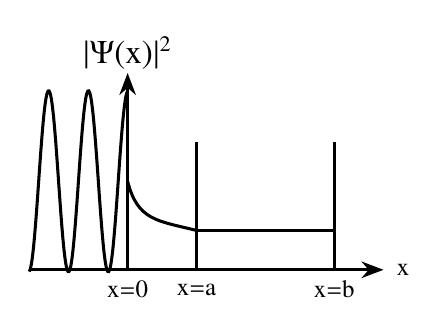
\begin{tikzpicture}[scale=0.5]
			\tikzstyle{every node}=[font=\large]
			\draw [line width=1.1pt, ->, >=Stealth] (11.75,12.75) -- (20.75,12.75);
			\draw [line width=1.1pt, ->, >=Stealth] (14.25,12.75) -- (14.25,17.75);
			\draw [line width=1.1pt, short] (16,12.75) -- (16,16);
			\draw [line width=1.1pt, short] (19.5,12.75) -- (19.5,16);
			\node [font=\small] at (19.5,12.25) {x=b};
			\node [font=\small] at (14.25,12.25) {x=0};
			\node [font=\small] at (16,12.25) {x=a};
			\node [font=\small] at (21.25,12.75) {x};
			\node [font=\large] at (14.25,18.25) {$\mid$$\Psi$(x)$\mid^{2}$};
			\draw[domain=11.75:14.25,samples=100,smooth, line width=1.1pt] plot (\x,{2.3*sin(6.22*\x r -11.75 r ) +15});
			\draw [line width=1.1pt, short] (14.25,15) .. controls (14.5,14) and (15,14) .. (16,13.75);
			\draw [line width=1.1pt, short] (16,13.75) -- (19.5,13.75);
		\end{tikzpicture}
		
		\item
		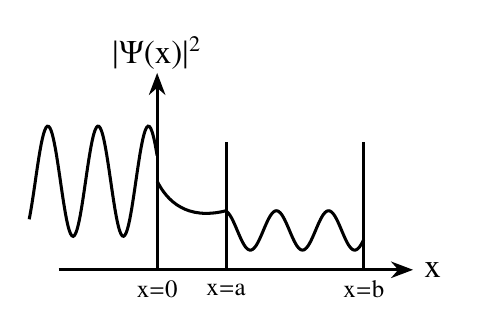
\begin{tikzpicture}[scale=0.5]
			\tikzstyle{every node}=[font=\large]
			\draw [line width=1.1pt, ->, >=Stealth] (11.75,12.75) -- (20.75,12.75);
			\draw [line width=1.1pt, ->, >=Stealth] (14.25,12.75) -- (14.25,17.75);
			\draw [line width=1.1pt, short] (16,12.75) -- (16,16);
			\draw [line width=1.1pt, short] (19.5,12.75) -- (19.5,16);
			\node [font=\small] at (19.5,12.25) {x=b};
			\node [font=\small] at (14.25,12.25) {x=0};
			\node [font=\small] at (16,12.25) {x=a};
			\node [font=\large] at (21.25,12.75) {x};
			\node [font=\large] at (14.25,18.25) {$\mid$$\Psi$(x)$\mid^{2}$};
			\draw[domain=11:14.25,samples=100,smooth, line width=1.1pt] plot (\x,{1.4*sin(4.92*\x r -10.9 r ) +15});
			\draw [line width=1.1pt, short] (14.25,15) .. controls (14.5,14.5) and (15,14) .. (16,14.25);
			\draw[domain=16:19.5,samples=100,smooth, line width=1.1pt] plot (\x,{0.5*sin(4.74*\x r -17.5 r ) +13.75});
		\end{tikzpicture}
	\end{enumerate}
\end{multicols}

\item The spin-orbit interaction term of an electron moving in a central field is written as \( f(r) \vec{l} \cdot \vec{s} \), where \( r \) is the radial distance of the electron from the origin. If an electron moves inside a uniformly charged sphere, then

\begin{multicols}{2}
	\begin{enumerate}
		\item[(A)] \( f(r) = \text{constant} \)
		\item[(B)] \( f(r) \propto r^{-1} \)
		\item[(C)] \( f(r) \propto r^{-2} \)
		\item[(D)] \( f(r) \propto r^{-3} \)
	\end{enumerate}
\end{multicols}

\item For the following circuit, the correct logic values for the entries $X_2$ and $Y_2$ in the truth table are \\
\begin{figure}[!ht]
	\centering
	\begin{minipage}{0.55\textwidth}
		\centering
		\resizebox{\textwidth}{!}{%
			\begin{circuitikz}
				\tikzstyle{every node}=[font=\LARGE]
				\draw (8.5,16) to[short] (8.75,16);
				\draw (8.5,15.5) to[short] (8.75,15.5);
				\draw (8.75,16) node[ieeestd and port, anchor=in 1, scale=0.89](port){} (port.out) to[short] (10.5,15.75);
				\draw (8.5,13) to[short] (8.75,13);
				\draw (8.5,12.5) to[short] (8.75,12.5);
				\draw (8.75,13) node[ieeestd and port, anchor=in 1, scale=0.89](port){} (port.out) to[short] (10.5,12.75);
				\draw (12.5,17.25) to[short] (12.75,17.25);
				\draw (12.5,16.75) to[short] (12.75,16.75);
				\draw (12.75,17.25) node[ieeestd or port, anchor=in 1, scale=0.89](port){} (port.out) to[short] (14.5,17);
				\draw (12.75,12.75) to[short] (13,12.75);
				\draw (12.75,12.25) to[short] (13,12.25);
				\draw (13,12.75) node[ieeestd or port, anchor=in 1, scale=0.89](port){} (port.out) to[short] (14.75,12.5);
				\draw (17,17) to[short] (17.25,17);
				\draw (17,16.5) to[short] (17.25,16.5);
				\draw (17.25,17) node[ieeestd nor port, anchor=in 1, scale=0.89](port){} (port.out) to[short] (19,16.75);
				\draw (18,13.5) to[short] (18.25,13.5);
				\draw (18,13) to[short] (18.25,13);
				\draw (18.25,13.5) node[ieeestd nor port, anchor=in 1, scale=0.89](port){} (port.out) to[short] (20,13.25);
				\draw [ line width=1.1pt](8.5,16) to[short] (6.75,16);
				\draw [ line width=1.1pt](8.5,15.5) to[short] (8.5,13);
				\draw [ line width=1.1pt](8.5,12.5) to[short] (6.5,12.5);
				\draw [ line width=1.1pt](6,14.25) to[short] (8.5,14.25);
				\draw [ line width=1.1pt](10.5,12.75) to[short] (13,12.75);
				\draw [ line width=1.1pt](12.75,12.25) to[short] (12.75,10.75);
				\draw [ line width=1.1pt](10.5,15.75) to[short] (10.5,16.75);
				\draw [ line width=1.1pt](10.5,16.75) to[short] (12.75,16.75);
				\draw [ line width=1.1pt](12.5,17.25) to[short] (12.5,18.5);
				\draw [ line width=1.1pt](14.75,12.5) to[short] (14.75,13);
				\draw [ line width=1.1pt](14.75,13) to[short] (18,13);
				\draw [ line width=1.1pt](14.5,17) to[short] (17,17);
				\draw [ line width=1.1pt](17,16.5) to[short] (17,15.25);
				\draw [ line width=1.1pt](17,15.25) to[short] (21.25,15.25);
				\draw [ line width=1.1pt](20,13.25) to[short] (21.25,13.25);
				\draw [ line width=1.1pt](21.25,15.25) to[short] (21.25,13.25);
				\draw [ line width=1.1pt](19,16.75) to[short] (20.75,16.75);
				\draw [ line width=1.1pt](18,13.5) to[short] (18,15);
				\draw [ line width=1.1pt](18,15.5) to[short] (19.75,15.5);
				\draw [ line width=1.1pt](19.75,15.5) to[short] (19.75,16.75);
				\draw [ line width=1.1pt](21.25,13.25) to[short] (22,13.25);
				\node at (21.25,13.25) [circ] {};
				\node at (19.75,16.75) [circ] {};
				\node at (12.75,10.75) [circ] {};
				\node at (12.5,18.5) [circ] {};
				\node at (8.5,14.25) [circ] {};
				\draw [line width=1.1pt, short] (18,15) .. controls (17.5,15) and (17.5,15.25) .. (18,15.5);
				\node [font=\LARGE] at (6,16) {A};
				\node [font=\LARGE] at (5.75,12.5) {B};
				\node [font=\LARGE] at (5.5,14.25) {G};
				\node [font=\LARGE] at (12.5,19.25) {C};
				\node [font=\LARGE] at (12.75,10.25) {P};
				\node [font=\LARGE] at (21,16.75) {X};
				\node [font=\LARGE] at (22.5,13.25) {Y};
			\end{circuitikz}
		}%
	\end{minipage}%
	\hfill
	\begin{minipage}{0.4\textwidth}
		\centering
		\begin{tabular}{|c|c|c|c|c|c|c|}
			\hline
			G & A & B & P & C & X & Y \\
			\hline
			1 & 0 & 1 & 0 & 0 & 0 & 1 \\
			0 & 0 & 0 & 1 & 1 & $X_2$ & $Y_2$ \\
			1 & 0 & 0 & 0 & 1 & 0 & 1 \\
			\hline
		\end{tabular}
	\end{minipage}
\end{figure}

\begin{multicols}{4}
	\begin{enumerate}
		\item 1 and 0
		\item 0 and 0
		\item 0 and 1
		\item 1 and 1
	\end{enumerate}
\end{multicols}
	
\item In a set of $N$ successive polarizers, the $m^{\text{th}}$ polarizer makes an angle $\left( \frac{m \pi}{2N} \right)$ with the vertical. A vertically polarized light beam of intensity $I_0$ is incident on two such sets with $N = N_1$ and $N = N_2$, where $N_2 > N_1$. Let the intensity of light beams coming out be $I(N_1)$ and $I(N_2)$, respectively. Which of the following statements is correct about the two outgoing beams?
	\begin{enumerate}
		\item $I(N_2) > I(N_1)$ ; the polarization in each case is vertical
		\item $I(N_2) < I(N_1)$ ; the polarization in each case is vertical
		\item $I(N_2) > I(N_1)$ ; the polarization in each case is horizontal
		\item $I(N_2) < I(N_1)$ ; the polarization in each case is horizontal
	\end{enumerate}

\item A ball bouncing off a rigid floor is described by the potential energy function\\
\begin{center}
	V$\brak{x}$ = $mgx$ for $x>0$\\
	= $\infty$ for $x \leq 0$
\end{center}
Which of the following schematic diagrams best represents the phase space plot of the ball?
\begin{multicols}{2}
	\begin{enumerate}
		\item 
		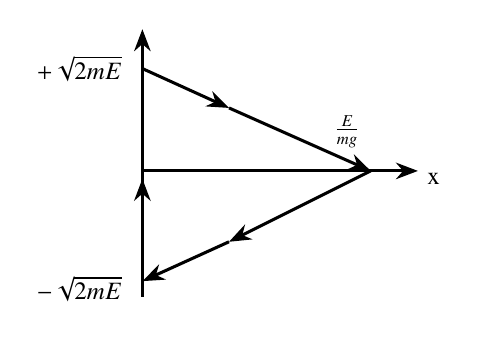
\begin{tikzpicture}[scale = 0.4]
			\tikzstyle{every node}=[font=\small]
			\draw [line width=1.1pt, ->, >=Stealth] (9.25,9.5) -- (9.25,18);
			\draw [line width=1.1pt, ->, >=Stealth] (9.25,13.5) -- (18,13.5);
			\draw [line width=1.1pt, ->, >=Stealth] (9.25,16.75) -- (12,15.5);
			\draw [line width=1.1pt, ->, >=Stealth] (12,15.5) -- (16.5,13.5);
			\draw [line width=1.1pt, ->, >=Stealth] (16.5,13.5) -- (12,11.25);
			\draw [line width=1.1pt, ->, >=Stealth] (12,11.25) -- (9.25,10);
			\draw [line width=1.1pt, ->, >=Stealth] (9.25,13) -- (9.25,13.25);
			\node [font=\small] at (18.5,13.25) {x};
			\node [font=\small] at (15.75,14.75) {$\frac{E}{mg}$};
			\node [font=\small] at (7.25,16.75) {$+\sqrt{2mE}$};
			\node [font=\small] at (7.25,9.75) {$-\sqrt{2mE}$};
		\end{tikzpicture}
		
		\item
		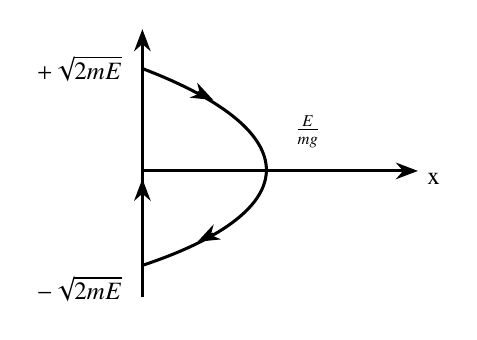
\begin{tikzpicture}[scale=0.4]
			\tikzstyle{every node}=[font=\small]
			\draw [line width=1.1pt, ->, >=Stealth] (9.25,9.5) -- (9.25,18);
			\draw [line width=1.1pt, ->, >=Stealth] (9.25,13.5) -- (18,13.5);
			\draw [line width=1.1pt, ->, >=Stealth] (9.25,13) -- (9.25,13.25);
			\node [font=\small] at (18.5,13.25) {x};
			\node [font=\small] at (14.5,14.75) {$\frac{E}{mg}$};
			\node [font=\small] at (7.25,16.75) {$+\sqrt{2mE}$};
			\node [font=\small] at (7.25,9.75) {$-\sqrt{2mE}$};
			\draw [line width=1.1pt, short] (9.25,16.75) .. controls (14.5,14.75) and (14.5,12.25) .. (9.25,10.5);
			\draw [line width=1.1pt, ->, >=Stealth] (11,16) -- (11.5,15.75);
			\draw [line width=1.1pt, ->, >=Stealth] (11.5,11.5) -- (11,11.25);
		\end{tikzpicture}
		
		\item
		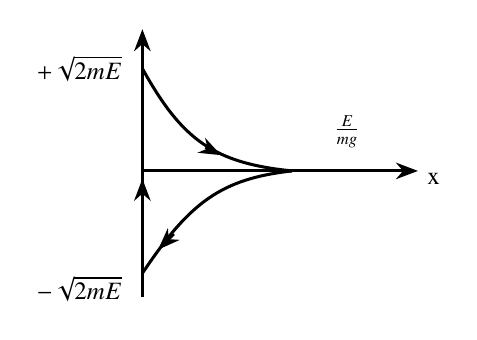
\begin{tikzpicture}[scale=0.4]
			\tikzstyle{every node}=[font=\small]
			\draw [line width=1.1pt, ->, >=Stealth] (9.25,9.5) -- (9.25,18);
			\draw [line width=1.1pt, ->, >=Stealth] (9.25,13.5) -- (18,13.5);
			\draw [line width=1.1pt, ->, >=Stealth] (9.25,13) -- (9.25,13.25);
			\node [font=\small] at (18.5,13.25) {x};
			\node [font=\small] at (15.75,14.75) {$\frac{E}{mg}$};
			\node [font=\small] at (7.25,16.75) {$+\sqrt{2mE}$};
			\node [font=\small] at (7.25,9.75) {$-\sqrt{2mE}$};
			\draw [line width=1.1pt, short] (9.25,16.75) .. controls (10.5,14.5) and (11.5,13.75) .. (14,13.5);
			\draw [line width=1.1pt, short] (14,13.5) .. controls (11.75,13.25) and (10.75,12.5) .. (9.25,10.25);
			\draw [line width=1.1pt, ->, >=Stealth] (11.25,14.25) -- (11.75,14);
			\draw [line width=1.1pt, ->, >=Stealth] (10.25,11.5) -- (9.75,11);
		\end{tikzpicture}
		
		\item
		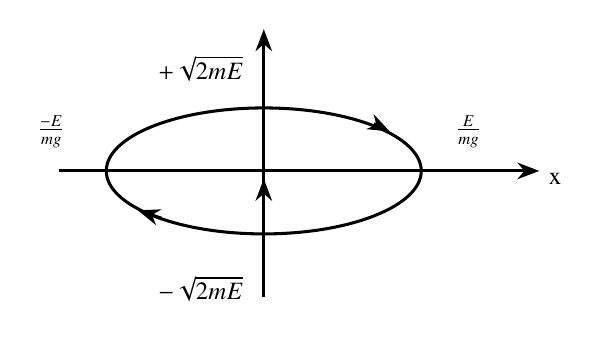
\begin{tikzpicture}[scale=0.4]
			\tikzstyle{every node}=[font=\small]
			\draw [line width=1.1pt, ->, >=Stealth] (9.25,9.5) -- (9.25,18);
			\draw [line width=1.1pt, ->, >=Stealth] (9.25,13) -- (9.25,13.25);
			\node [font=\small] at (18.5,13.25) {x};
			\node [font=\small] at (15.75,14.75) {$\frac{E}{mg}$};
			\node [font=\small] at (7.25,16.75) {$+\sqrt{2mE}$};
			\node [font=\small] at (7.25,9.75) {$-\sqrt{2mE}$};
			\draw [line width=1.1pt, ->, >=Stealth] (2.75,13.5) -- (18,13.5);
			\draw [ line width=1.1pt ] (9.25,13.5) ellipse (5cm and 2cm);
			\node [font=\small] at (2.5,14.75) {$\frac{-E}{mg}$};
			\draw [line width=1.1pt, ->, >=Stealth] (12.75,15) -- (13.25,14.75);
			\draw [line width=1.1pt, ->, >=Stealth] (6,12) -- (5.25,12.25);
		\end{tikzpicture}
	\end{enumerate}
\end{multicols}

\item An infinitely long wire parallel to the $x-axis$ is kept at $z=d$ and carries a current $I$ in the positive $x$ direction above a superconductor filling the region $z \leq 0$ (see figure). The magnetic field $\overrightarrow{B}$ inside the superconductor is zero so that the field just outside the superconductor is parallel to its surface. The magnetic field due to this configuration at a point $\brak{x,y,z>0}$ is\\
\begin{figure}[!ht]
	\centering
	\resizebox{0.5\textwidth}{!}{%
		\begin{circuitikz}
			\tikzstyle{every node}=[font=\LARGE]
			\draw [->, >=Stealth] (6.5,11.25) -- (17.5,11.25);
			\draw [->, >=Stealth] (10.5,11.25) -- (10.5,17);
			\draw [->, >=Stealth] (5.5,13.25) -- (19,13.25);
			\node [font=\LARGE] at (19.25,13.75) {I};
			\draw [<->, >=Stealth] (11.5,13.25) -- (11.5,11.25);
			\node [font=\LARGE] at (12,12) {d};
			\node [font=\LARGE] at (18,11.25) {$\hat{x}$};
			\node [font=\large] at (10.5,9.5) {superconductor};
			\draw [line width=1pt, short] (7.25,11.25) -- (6.5,10.5);
			\draw [line width=1pt, short] (8.25,11.25) -- (6.5,9.5);
			\draw [line width=1pt, short] (9.25,11.25) -- (6.5,8.5);
			\draw [line width=1pt, short] (10.25,11.25) -- (6.5,7.25);
			\draw [line width=1pt, short] (11.25,11.25) -- (10,9.75);
			\draw [line width=1.1pt, short] (9.75,9.25) -- (8,7.25);
			\draw [line width=1.1pt, short] (12.25,11.25) -- (11.25,9.75);
			\draw [line width=1.1pt, short] (11,9.25) -- (9.25,7.25);
			\draw [line width=1.1pt, short] (13.75,11.25) -- (10.75,7.25);
			\draw [line width=1.1pt, short] (15,11.25) -- (12.25,7.25);
			\draw [line width=1.1pt, short] (16,11.25) -- (13.5,7.25);
			\draw [line width=1.1pt, short] (17,11.25) -- (14.75,7.25);
			\draw [line width=1.1pt, short] (17.25,9.75) -- (16,7.25);
			\draw [line width=1.1pt, short] (17.25,8) -- (17,7.25);
			\node [font=\LARGE] at (9.75,17) {$\hat{z}$};
		\end{circuitikz}
	}%
\end{figure}

\begin{enumerate}
	\item $\brak{\frac{\mu_0 I}{2\pi}} \frac{-(z-d)\hat{j} + y\hat{k}}{[y^{2}+(z-d)^{2}]}$
	\item $\brak{\frac{\mu_0 I}{2\pi}} \brak{\frac{-(z-d)\hat{j} + y\hat{k}}{[y^{2}+(z-d)^{2}]} + \frac{(z+d)\hat{j} - y\hat{k}}{[y^{2}+(z+d)^{2}]}}$
	\item $\brak{\frac{\mu_0 I}{2\pi}} \brak{\frac{-(z-d)\hat{j} + y\hat{k}}{[y^{2}+(z-d)^{2}]} - \frac{(z+d)\hat{j} - y\hat{k}}{[y^{2}+(z+d)^{2}]}}$
	\item $\brak{\frac{\mu_0 I}{2\pi}} \brak{\frac{y\hat{j} + (z-d)\hat{k}}{[y^{2}+(z-d)^{2}]} + \frac{y\hat{j} - (z+d)\hat{k}}{[y^{2}+(z+d)^{2}]}}$
\end{enumerate}

\item The vector potential inside a long solenoid, with n turns per unit length and carrying current I, written in cylindrical coordinates is $\overrightarrow{A}\brak{s,\phi,z} = \frac{\mu_0nI}{2} s \hat{\phi}$. If the term $\frac{\mu_0nI}{2} s\brak{\alpha\cos{\phi}\hat{\phi} + \beta\sin{\phi}\hat{s}}$, where $\alpha \neq 0$, $\beta \neq 0$, is added to $A\brak{s,\phi,z}$, the magnetic field remains the same if
\begin{multicols}{4}
\begin{enumerate}
	\item $\alpha = \beta$
	\item $\alpha = -\beta$
	\item $\alpha = 2\beta$
	\item $\alpha = \frac{\beta}{2}$ 
\end{enumerate}
\end{multicols}

\begin{center}
$
\brak{
\begin{array}{l}
	\text{Useful formulae:} \quad \vec{v} = \frac{\partial t}{\partial s} \hat{s} + \frac{1}{s} \frac{\partial t}{\partial \phi} \hat{\phi} + \frac{\partial t}{\partial z} \hat{z} ; \\[10pt]
	\vec{\nabla} \times \vec{v} = \left( \frac{1}{s} \frac{\partial v_z}{\partial \phi} - \frac{\partial v_{\phi}}{\partial z} \right) \hat{s} + \left( \frac{\partial v_s}{\partial z} - \frac{\partial v_z}{\partial s} \right) \hat{\phi} + \frac{1}{s} \left( \frac{\partial (s v_{\phi})}{\partial s} - \frac{\partial v_s}{\partial \phi} \right) \hat{z}
\end{array}
}
$
\end{center} 

\item Low energy collision (s-wave scattering) of pion ($\pi^+$) with deuteron ($d$) results in the production of two protons ($\pi^+ + d \rightarrow p + p$). The relative orbital angular momentum (in units of $\hbar$) of the resulting two-proton system for this reaction is
\begin{multicols}{4}
\begin{enumerate} 
	\item 0
	\item 1
	\item 2
	\item 3
\end{enumerate}
\end{multicols}

\item Consider the Hamiltonian $ H(q, p) = \frac{\alpha p^2 q^4}{2} + \frac{\beta}{q^2} $, where $\alpha$ and $\beta$ are parameters with appropriate dimensions, and $q$ and $p$ are the generalized coordinate and momentum, respectively. The corresponding Lagrangian $L(q, \dot{q})$ is
\begin{multicols}{4}
\begin{enumerate}
	\item $ \frac{1}{2 \alpha} \frac{\dot{q}^2}{q^{4}} - \frac{\beta}{q^2} $
	\item $\frac{2}{\alpha} \frac{\dot{q}^2}{q^{4}} + \frac{\beta}{q^2}$
	\item $\frac{1}{\alpha} \frac{\dot{q}^2}{q^{4}} + \frac{\beta}{q^2}$
	\item $ -\frac{1}{2 \alpha} \frac{\dot{q}^2}{q^{4}} + \frac{\beta}{q^2}$
\end{enumerate}
\end{multicols}

\end{enumerate}
\end{document}


